\chapter{Comparing Algorithms}


\section{Time Analysis}

here how much time they take, in p,k and n give approximate O(x) value

\begin{Schunk}
\begin{Sinput}
>     library(norMmix, lib.loc="~/ethz/BA/norMmix.Rcheck/")
>     savdir <- normalizePath("~/ethz/BA/Rscripts/2time")
>     filelist <- list.files(savdir, pattern=".rds")
>     filelist <- grep("mcl.rds", filelist, invert=TRUE, value=TRUE)
>     f <- lapply(file.path(savdir,filelist), function(j) readRDS(j)$fit)
>     times <- unlist(lapply(f, function(j) extracttimes(j)[,,1]))
>     dims <- unlist(lapply(f, function(j) attr(extracttimes(j), "p")))
>     size <- unlist(lapply(f, function(j) attr(extracttimes(j), "n")))
>     ddims <- rep(dims, each=80)
>     ssize <- rep(size, each=80)
>     pars <- unlist(lapply(f, npar))
>     r <- lm(log(times) ~ log(pars) + log(ddims) + log(ssize))
>     summary(r)
\end{Sinput}
\begin{Soutput}
Call:
lm(formula = log(times) ~ log(pars) + log(ddims) + log(ssize))

Residuals:
    Min      1Q  Median      3Q     Max 
-3.4428 -0.2986  0.0671  0.4579  2.0936 

Coefficients:
            Estimate Std. Error t value Pr(>|t|)    
(Intercept) -9.74133    0.10598  -91.91   <2e-16 ***
log(pars)    2.75983    0.01181  233.75   <2e-16 ***
log(ddims)  -2.06063    0.02483  -82.99   <2e-16 ***
log(ssize)   0.61301    0.01446   42.38   <2e-16 ***
---
Signif. codes:  0 ‘***’ 0.001 ‘**’ 0.01 ‘*’ 0.05 ‘.’ 0.1 ‘ ’ 1

Residual standard error: 0.6946 on 7196 degrees of freedom
Multiple R-squared:  0.8887,	Adjusted R-squared:  0.8887 
F-statistic: 1.916e+04 on 3 and 7196 DF,  p-value: < 2.2e-16
\end{Soutput}
\end{Schunk}

\begin{figure}[h]
    \centering
\begin{Schunk}
\begin{Sinput}
>     plot(times~pars, log="xy", yaxt="n", xaxt="n")
>     sfsmisc::eaxis(1)
>     sfsmisc::eaxis(2)
\end{Sinput}
\end{Schunk}
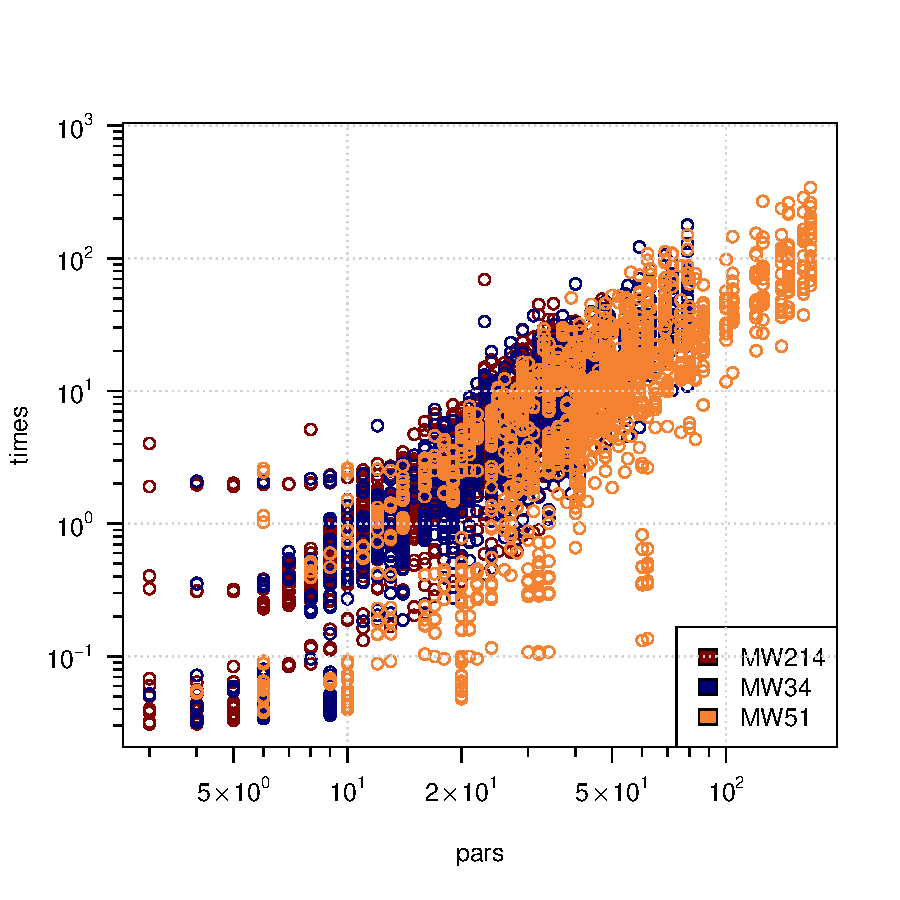
\includegraphics{chapter3-figtime}
    \caption{Log-log Plot of System Time against Parameter Length}
    \label{fig:time}
\end{figure}

can see that time is almost one to one proportional to parameter length.

\section{Behaviour in {\tt n}}

% it 1
here show as expected narrower scattering as n increases

\section{Behaviour in {\tt p}}

% it 1
here show how norMmix is consistently competitive with mclust

\section{Diffixult Mixtures}

% it 1
here show behaviour in difficult cases

\section{Nonnormal mixtures}

